La comunicación entre contenedores presenta dos formas posibles:

\begin{enumerate}
    \item O bien mediante la comunicación mediante una red o un \textit{socket}.
    \item O bien mediante ficheros compartidos en un volúmen o carpeta.
\end{enumerate}

Evidentemente, cada una presenta sus ventajas. Sin embargo, la primera opción es la
escogida por lo general. ¿Por qué?

Habilitar la comunicación mediante una red asegura que solo los contenedores
especificados reciben la información en cuestión. Si se usa un directorio compartido
se corre el riesgo de que otra aplicación pueda ver la información y eso no es seguro.

Por otra parte, las comunicaciones vía red facilitan la escucha pasiva mediante el
uso de puertos: si se tiene un puerto publicado, basta con escuchar allí a la
espera de peticiones. Si se pretende realizar una comunicación mediante un
directorio compartido es necesario o bien hacer \textit{polling} cada `x' segundos
o bien usar algún mecanismo del kernel (como \texttt{inotify}) para ser notificados
cuando se realice alguna acción sobre un fichero en cuestión.

Finalmente, comunicaciones basadas en la red permiten identificar quién es el
emisor que está al otro lado, escuchando o recibiendo información. Sin embargo, en
comunicaciones basadas en ficheros cualquiera puede acceder y no se sabe necesariamente
qué proceso es el último que ha editado o leído un fichero.

La forma de comunicar dos contenedores vía red se realiza principalmente mediante
puentes (conexiones tipo \textit{bridge}). Este tipo de interfaz es nativa de Docker
y muy fácil de configurar. Por defecto, un contenedor usará este tipo de red para
realizar sus comunicaciones con el exterior y con otros equipos, por lo que
usarla para conectar varios contenedores es sencillo. Existen dos formas de hacerlo:

\begin{enumerate}
    \item Durante la creación, especificando la red a la que conectarse.
    \item En tiempo de ejecución, usando el cliente Docker para indicarle a un
          contenedor que se debe unir a una red.
\end{enumerate}

\subsubsection*{Conexión}
Para realizar la conexión entre contenedores se utilizan siempre redes virtuales.
El tipo de red puede variar según se necesite, pero principalmente se usan las
tipo puente (mencionadas anteriormente) y las redes \textit{overlay}, más específicas
para casos más concretos que se mencionarán más adelante.

En estas redes el contenedor cuenta con una dirección IP única asignada por el servicio
Docker (\texttt{dockerd}) y, opcionalmente, un \textit{hostname} que permite la
identificación directa y sencilla del contenedor.

Por defecto, Docker crea una interfaz \textit{bridge} para el contenedor y se puede
usar para comunicar dos contenedores. Sin embargo, el nombre de las redes no es
fácilmente accesible y menos el de los contenedores. La idea principal radica en
el uso de la IP única asignada a dicha interfaz: si se obtiene la dirección de
un contenedor, otro podrá enviar información directamente a esa IP.

La forma de configurar esta conexión es la siguiente:

\begin{enumerate}
    \item Se comprueba que la red a la que se quieran conectar los contenedores esté
          en ejecución. Esto se consigue gracias al comando \lstinline[style=bash]!docker network ls!:
          \begin{figure}[H]
              \centering
              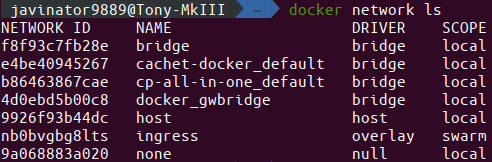
\includegraphics[width=.6\linewidth]{pictures/network-ls.png}
          \end{figure}

    \item Se inician los contenedores (o se obtiene su ID) para posteriormente, poder
          obtener su IP. Se puede obtener el identificador de un contenedor mediante
          el comando \lstinline[style=bash]!docker container ls!:
          \begin{figure}[H]
              \centering
              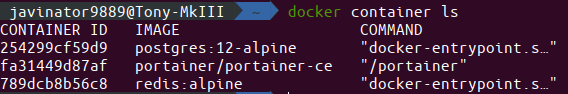
\includegraphics[width=.5\linewidth]{pictures/container-ls.png}
          \end{figure}

    \item Finalmente, se obtiene la dirección IP interna del contenedor. Para ello,
          se pueden usar herramientas externas como \href{https://www.portainer.io/}{Portainer}
          o directamente desde el terminal mediante comandos: \lstinline[style=bash]!docker inspect <container-id> | grep IPAddress!:
          \begin{figure}[H]
              \centering
              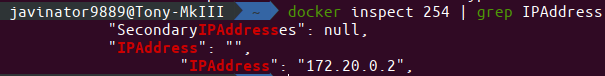
\includegraphics[width=.5\linewidth]{pictures/ip-address.png}
          \end{figure}
\end{enumerate}

Con la dirección IP ya podemos empezar a comunicarnos con el contenedor, tanto
desde dentro de Docker como desde la máquina anfitriona. Esto se puede comprobar
fácilmente haciendo un \texttt{ping} a la IP (figura \ref{fig:ping}):

\begin{figure}[H]
    \centering
    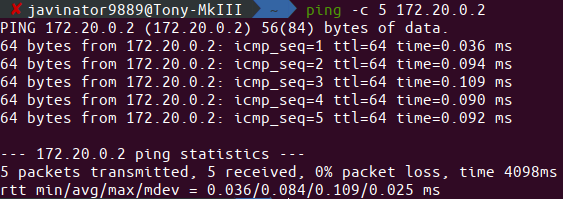
\includegraphics[width=.6\linewidth]{pictures/container-ping.png}
    \caption{Desde la máquina anfitriona nos podemos comunicar con el contenedor mediante la IP.}
    \label{fig:ping}
\end{figure}

\noindent\rule{\linewidth}{.2pt}

La opción anterior sin embargo es bastante tediosa y no permite realizarlo fácilmente
en pocas líneas. Es por ello por lo que existe la opción de redes definidas por el
usuario (\textit{user-defined bridge network} \cite{donohueHowCommunicateDocker2020}).

Cuando un grupo de contenedores se unen a una red tipo puente definida por el usuario
ya no es necesario tener el control sobre la dirección IP de cada contenedor
sino que basta con referenciar al contenedor por su nombre (figura \ref{fig:user-defined-network}):

\begin{figure}[H]
    \centering
    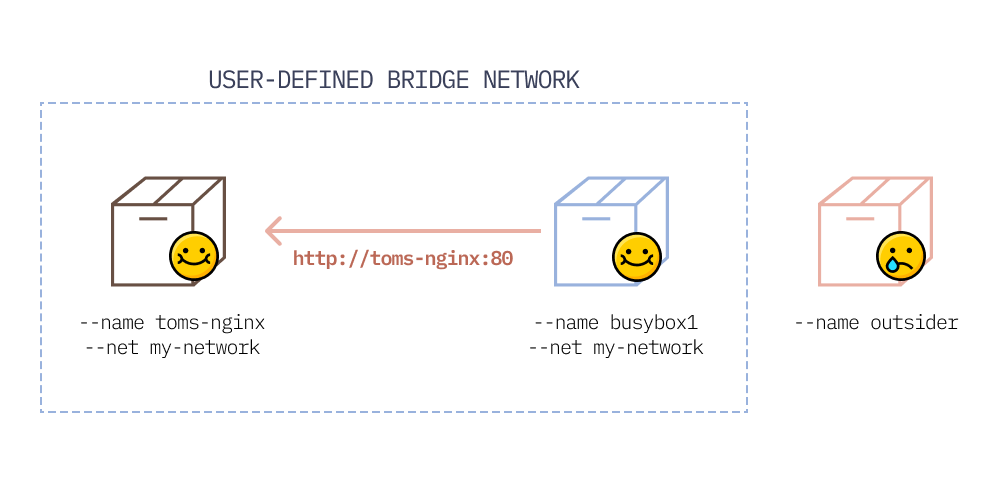
\includegraphics[width=.7\linewidth]{pictures/user-defined-bridge.png}
    \caption{Interfaz de red tipo puente definida por el usuario para facilitar la comunicación entre contenedores \cite{donohueHowCommunicateDocker2020}.}
    \label{fig:user-defined-network}
\end{figure}

De esta forma, si se ejecuta una base de datos dentro de un contenedor (por ejemplo,
una base tipo PostgreSQL), la conexión se puede realizar directamente escribiendo:

\begin{center}
    \texttt{postgresql://psql-container:5432}
\end{center}

\noindent lo cual facilita mucho la labor de depuración y desarrollo.

El proceso de creación y conexión en este caso es de la siguiente forma:

\begin{enumerate}
    \item Se crea una red definida por el usuario de tipo puente, mediante el
          comando \lstinline[style=bash]!docker network create <name>!. Por debajo
          Docker se encargará de gestionar todo lo necesario:

          \begin{figure}[H]
              \centering
              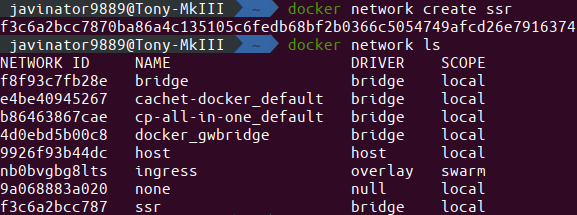
\includegraphics[width=.5\linewidth]{pictures/network-create.png}
          \end{figure}

    \item A continuación se crea el contenedor y se le asigna la red que acabamos
          de crear. Es importante en este paso asignarle también un nombre al
          contenedor para que sea fácilmente accesible. Lo primero se consigue
          con la opción \lstinline[style=bash]!--network <network-name>! y lo segundo
          con la directiva \lstinline[style=bash]!--name <container-name>!:
        
          \begin{figure}[H]
              \centering
              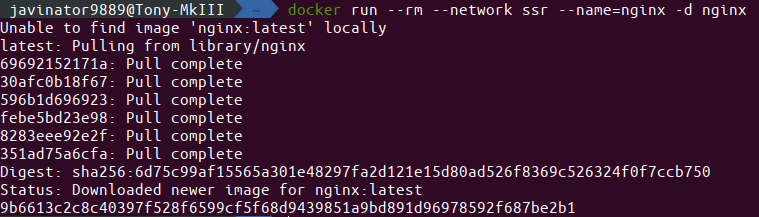
\includegraphics[width=.9\linewidth]{pictures/container-create.png}
          \end{figure}

    \item Finalmente, creamos el/los otro(s) contenedor(es) y les asociamos igualmente
          la red que hemos creado. En este caso, vamos a ejecutar una terminal
          básica que va a realizar una petición al servidor de NGINX que acabamos
          de levantar con el comando \texttt{wget}. Para acceder se pone directamente
          el nombre del contenedor de NGINX y el puerto al que se quiere acceder,
          no hace falta usar la IP:

          \begin{figure}[H]
              \centering
              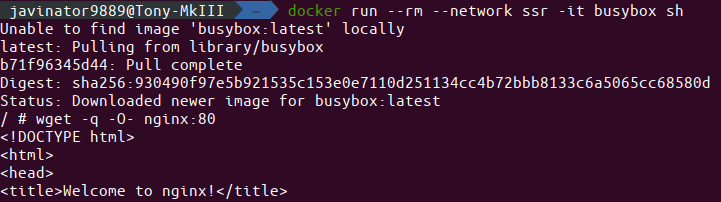
\includegraphics[width=.9\linewidth]{pictures/nginx-wget.png}
          \end{figure}
\end{enumerate}

Lo interesante de este método no es solo que no haga falta saber la IP del contenedor
(la cual entre reinicios puede cambiar) sino que además permite la conexión ``en caliente''
de un contenedor a la red: si durante la creación no le hemos asignado la red no habría
problema ya que existe un método de poder unir el contenedor a la red. Este comando
es \lstinline[style=bash]!docker network connect <network-name> <container-name/ID>!
y permite gestionar las interfaces de red de un contenedor fácilmente \cite{DockerNetworkConnect2021}.
Es el reemplazo del antiguo comando \texttt{-{}-link}, ya en deshuso \cite{LegacyContainerLinks2021}
el cual unía dos contenedores por medio de una red puente.

\subsubsection*{Redes \textit{overlay}}
Otra forma de conectar contenedores es mediante las redes \textit{overlay}. 
Dichas redes permiten conectar múltiples clústers de Docker (en particular, \textit{Swarm})
entre sí para facilitar el intercambio de información. Sin embargo, el modo de
funcionamiento ya no se limita únicamente a una red local sino a una red WAN para la
que es necesario añadir orquestación mediante Kubernetes o Docker Swarm.

El procedimiento sin embargo es muy similar al de crear una red tipo puente personalizada,
solo se alteran algunos pasos:

\begin{enumerate}
    \item Inicializamos un clúster de \textit{Swarm} y exponemos la IP a la cual otros
          nodos podrán unirse. Esto se hace con:

          \begin{center}
              \lstinline[style=bash]!docker swarm init --advertise-addr <IP-address>!
          \end{center}

    \item Tras la creación se generará un token el cual se usará para unirse al
          clúster de Swarm:

          \begin{center}
              \lstinline[style=bash]!docker swarm join --token <Swarm-token>!
          \end{center}

          Este paso es necesario ya que, en otro caso, estaremos trabajando sobre
          el servicio local de Docker y no sobre el clúster de Swarm.

    \item A continuación, creamos la red \textit{overlay}. En este caso, el comando
          difiere en que hay que añadir el tipo de red que se quiere crear:

          \begin{center}
              \lstinline[style=bash]!docker network create -d overlay <network-name>!
          \end{center}

          \begin{figure}[H]
              \centering
              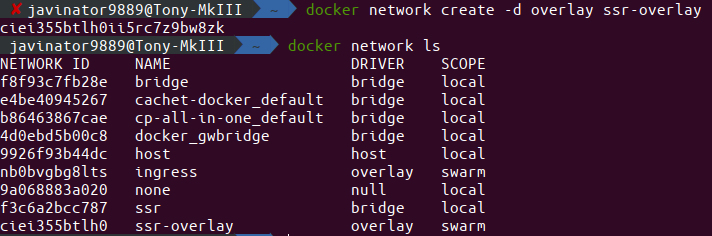
\includegraphics[width=.6\linewidth]{pictures/network-create-overlay.png}
          \end{figure}

    \item Como se está trabajando sobre Docker Swarm, se han de crear servicios
          (no contenedores) que se ejecutarán de forma distribuida a lo largo del
          clúster. En este caso, a modo de demostración se va a crear un servicio
          de NGINX que sea similar al del ejemplo anterior:

          \begin{center}
              \lstinline[style=bash]!docker service create --name nginx-server -d --network ssr-overlay nginx!
          \end{center}

          \begin{figure}[H]
              \centering
              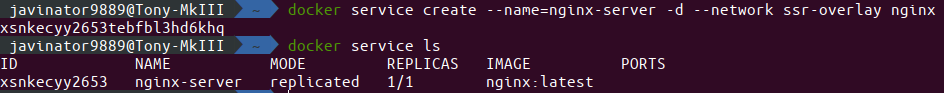
\includegraphics[width=.6\linewidth]{pictures/nginx-service-create.png}
          \end{figure}

    \item Finalmente, se crea otro servicio que en este caso va a acceder directamente
          al servicio de NGINX mediante el comando \texttt{wget}:

          \begin{center}
              \lstinline[style=bash]!docker service create --network ssr-overlay --name bb -d busybox wget -q -O- nginx-server:80!
          \end{center}

          \begin{figure}[H]
              \centering
              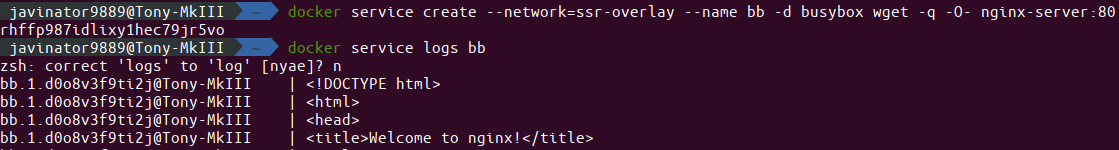
\includegraphics[width=.9\linewidth]{pictures/nginx-wget-swarm.png}
          \end{figure}
\end{enumerate}

Como se puede ver, también se pueden conectar los contenedores a través de redes 
\textit{overlay} y usando directamente el nombre del contenedor. Su configuración
es bastante más compleja y añade más pasos, que se explicarán con más detalle
en el punto \ref{sec:swarm}.